% !TeX encoding = UTF-8
% !TeX program = xelatex
% !TeX spellcheck = en_US

\documentclass[a4paper]{ltxdoc}
\usepackage{amsmath}
\usepackage[UTF8]{ctex}
\usepackage{unicode-math}
\usepackage{caption}
\usepackage{booktabs}
\usepackage{xcolor}
\usepackage{array}
\usepackage{listings}
\usepackage[perpage]{footmisc}
\usepackage{hypdoc}
\usepackage{geometry}
\usepackage{endnotes}
\usepackage{graphicx}
% \usepackage[multiple]{endnotes}
\usepackage{multicol}
\usepackage{blindtext}
\geometry{a4paper, scale=0.85}
\newenvironment{Figure}
{\par\medskip\noindent\minipage{\linewidth}}
{\endminipage\par\medskip}

\title{实验报告\\半导体温度计}
\author{少年班学院\\马天开 PB21000030(5号)}
\date{\today}

\begin{document}
\begin{multicols}{2}
    \maketitle
    \section{实验目的}
    利用半导体热敏电阻的阻值随温度变化的特性,利用非定量电测法,设计制作半导体温度计,进行温度的测量。

    同时,学习基本的电学实验操作和电烙铁的使用流程,掌握简单的电路设计和实验数据处理能力。

    \section{实验原理}
    实验中使用的热敏电阻器是以锰、钴、镍、铜等对温度敏感的金属氧化物制成的元件,这类元件在温度较低时,电子受束缚,载流子数量少,阻值较高。随着温度升高,原子热运动家具,部分电子获得更高额能量,变成自由电子,在原位留下空穴,增强了半导体的导电能力。

    一般来说,负温度系数热敏电阻的电阻和温度满足如下关系:

    \begin{equation}
        R_T = R_{\infty} e^{\frac{B}{T}}
    \end{equation}
    其中$T$为热力学温度,$R_T$为在温度$T$下对应的热敏电阻阻值,$R_{\infty}$为$T\to \infty$时热敏电阻的阻值,$B$为一常数,记作热敏电阻的材料系数。

    另外,热敏电阻在电流较大时并不符合欧姆定律,此时表现出明显的非线性。在实验中要保证较小的电流来确保热敏电阻上散失的功率不足以显著地改变热敏电阻的温度,此时电阻近似符合欧姆定律。

    在本实验中,设计一平衡电桥对其阻值进行测量,其中各项参数的选取主要需要参考以下内容:

    在温度下限$T_1 = 20^{\circ}C$时,要求电流表示数$I_g = 0$,此时热敏电阻阻值为$R_{T1}$,电桥的平衡条件为:$R_1/R_2 = R_3/R_T$,如果假设此时电桥为平衡电桥,取$R_1 = R_2$,则$R_3 = R_{T1}$。

    当达到温度上限$T_2 = 70^{\circ} C$时,电流表的读数应当满偏:$I_g = I_G$,此时,通过计算可以得到:

    \begin{equation}
        R_1 = \dfrac{2V_{CD}}{I_G}(\dfrac 1 2 - \dfrac{R_{T2}}{R_{T1} + R_{T2}}) - 2(R_G + \dfrac {R_{T1}R_{T2}}{R_{T1}+R_{T2}})
        \label{eq:R1}
    \end{equation}

    根据实验中使用的热敏电阻的特性,选取$V_{CD} = 1V$,并根据公式~\ref{eq:R1}计算$R_1$和$R_2$。

    \section{实验仪器}
    电烙铁、万用表、恒温水浴箱x2

    热敏电阻(温度特性给定)、电流计($R_g$已知)、可变电阻箱、电位器5个、$1.5V$电池、多档开关、待焊接的电路板、导线若干。

    \section{实验流程}
    \subsection{设计计算电路参数}

    根据数据,确定设计的半导体温度计温度下限对应的电阻值$R_{T1}$和上限对应电阻值$R_{T2}$,据此确定最大工作电流$I_T$。根据实验中采用的热敏电阻的实际情况,选取$V_{CD} = 1V$。选用$1.5V$干电池作为电源,并计算得到$R_1$和$R_2$的值。

    \subsection{连接电路和电路元件设定}

    在焊接电路前首先调节$R_1$和$R_2$,并用万用表测量,使其达到计算值,在之后的操作中保持$R_1$和$R_2$的值不变。

    用电烙铁焊接电路,焊接时$K1$放在1挡,电流计应该最后接入电路,防止电流过大损坏仪表。

    将开关置于3挡出,另电阻箱的阻值为$R_{T1}$,调节$R_3$的值,使电表示数为0,在之后的操作保持$R_3$不变。

    然后,将电阻箱的阻值调为$R_{T2}$,调节$R$的值,使电表满偏。

    开关置于2挡,调节电位器$R_4$使电表满偏。

    \subsection{标定刻度}

    开关置于3挡,每隔$5^{\circ}C$将热敏电阻的电阻-温度特性曲线上读取一系列的电阻值,分别对应到电表上的示数,分别记录下来。

    \subsection{安装热敏电阻}

    开关置于1挡,用热敏电阻替代电阻箱,再将开关置于3挡。

    \subsection{测试}

    用此温度计测量两恒温水箱的读数,与水银温度计的示数做比较,计算测量的相对误差。

    \section{实验数据}

    \subsection{原始数据}

    实验中记录到的数据如下:

    \begin{Figure}
        \centering
        \begin{tabular}{|c|c|}
            \hline
            \textbf{$T/{}^{\circ}C$} & \textbf{$I/\mu A$} \\\hline
            20                       & 0.0                \\\hline
            25                       & 6.7                \\\hline
            30                       & 12.9               \\\hline
            35                       & 19.4               \\\hline
            40                       & 24.3               \\\hline
            45                       & 30.2               \\\hline
            50                       & 34.8               \\\hline
            55                       & 39.7               \\\hline
            60                       & 43.7               \\\hline
            65                       & 46.3               \\\hline
            70                       & 50.0               \\\hline
        \end{tabular}
    \end{Figure}
    另外测量得到两个恒温箱的数据分别为:

    \begin{Figure}
        \centering
        \begin{tabular}{|c|c|}
            \hline
            \textbf{$T/{}^{\circ}C$} & \textbf{$I/\mu A$} \\\hline
            32.5                     & 14.5               \\\hline
            57.4                     & 42.7               \\\hline
        \end{tabular}
    \end{Figure}

    \subsection{数据处理}

    对于测量的数据,首先做出温度——电流图像如下:
    \begin{Figure}
        \centering
        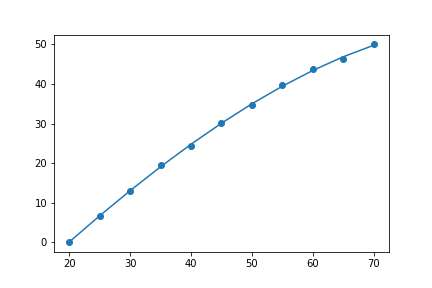
\includegraphics[scale = 0.3]{img/1.png}
    \end{Figure}

    图中曲线为三次拟合的结果,以此曲线为基础,取其逆函数,计算$I = 14.5\mu A$对应的温度值,计算为:$31.21^{\circ}C$,相对误差$\omega = 0.9\%$;同样的,计算$I = 42.7\mu A$对应的温度值,计算为:$58.06^{\circ}C$,相对误差$\omega = 1.1\%$

    \section{总结}

    \subsection{实验结论}

    见数据处理部分。

    \subsection{误差来源}

    主要误差来源出在温度——电流曲线上,此曲线采样频率不高,因此拟合精度不足,此外其他电学元件的内阻同样会对实验结果产生误差。

    可能的改进方法:选用精度更高的电流计、提高采样频率。

    \subsection{思考题}

    \begin{itemize}
        \item  用万用表测量并调整$R_1$和$R_2$的阻值时,为什么可以取比计算值略小的整数。为什么?

              注意到两个电阻接入电路的导线也存在电阻值,因此精度的要求应该适当放低,取比计算值略小的整数可以平衡这一误差。

        \item 完成电路连接后,如果要测$R_1$和$R_2$,为什么需将开关置于1挡,拔下E处接线、断开电流计?

              注意到上述操作是为了将两个电阻从电路中脱离开,以免受到电路其他部分的影响。。

        \item  开关置于3挡,电阻箱接入接线柱,使电阻箱的阻值为上限温度对应的$R_{T2}$,调节电位器$R$,使电流计满偏。为什么?

              上述操作是考虑到读取电流使最大化利用电流表上刻度,尽可能降低误差。

        \item 开关置于2挡,调节电位器$R_4$,使电流表满偏,这样做的目的是什么?

              为保证$R_4$等效替代上限温度的热敏电阻,满足实验原理。
    \end{itemize}
\end{multicols}
\end{document}